\documentclass[openany]{book}
\usepackage{lmodern}
\usepackage{amssymb,amsmath}
\usepackage{ifxetex,ifluatex}
\usepackage{fixltx2e} % provides \textsubscript
\ifnum 0\ifxetex 1\fi\ifluatex 1\fi=0 % if pdftex
  \usepackage[T1]{fontenc}
  \usepackage[utf8]{inputenc}
\else % if luatex or xelatex
  \ifxetex
    \usepackage{mathspec}
  \else
    \usepackage{fontspec}
  \fi
  \defaultfontfeatures{Ligatures=TeX,Scale=MatchLowercase}
\fi
% use upquote if available, for straight quotes in verbatim environments
\IfFileExists{upquote.sty}{\usepackage{upquote}}{}
% use microtype if available
\IfFileExists{microtype.sty}{%
\usepackage{microtype}
\UseMicrotypeSet[protrusion]{basicmath} % disable protrusion for tt fonts
}{}
\usepackage[margin=1in]{geometry}
\usepackage{hyperref}
\hypersetup{unicode=true,
            pdftitle={Spatial modelling of the electoral two-party preferred vote in Australia. A study of federal elections between 2001 and 2016 via the eechidna R package.},
            pdfauthor={Jeremy Forbes, Di Cook \& Rob Hyndman},
            pdfborder={0 0 0},
            breaklinks=true}
\urlstyle{same}  % don't use monospace font for urls
\usepackage{natbib}
\bibliographystyle{apalike}
\usepackage{longtable,booktabs}
\usepackage{graphicx,grffile}
\makeatletter
\def\maxwidth{\ifdim\Gin@nat@width>\linewidth\linewidth\else\Gin@nat@width\fi}
\def\maxheight{\ifdim\Gin@nat@height>\textheight\textheight\else\Gin@nat@height\fi}
\makeatother
% Scale images if necessary, so that they will not overflow the page
% margins by default, and it is still possible to overwrite the defaults
% using explicit options in \includegraphics[width, height, ...]{}
\setkeys{Gin}{width=\maxwidth,height=\maxheight,keepaspectratio}
\IfFileExists{parskip.sty}{%
\usepackage{parskip}
}{% else
\setlength{\parindent}{0pt}
\setlength{\parskip}{6pt plus 2pt minus 1pt}
}
\setlength{\emergencystretch}{3em}  % prevent overfull lines
\providecommand{\tightlist}{%
  \setlength{\itemsep}{0pt}\setlength{\parskip}{0pt}}
\setcounter{secnumdepth}{5}
% Redefines (sub)paragraphs to behave more like sections
\ifx\paragraph\undefined\else
\let\oldparagraph\paragraph
\renewcommand{\paragraph}[1]{\oldparagraph{#1}\mbox{}}
\fi
\ifx\subparagraph\undefined\else
\let\oldsubparagraph\subparagraph
\renewcommand{\subparagraph}[1]{\oldsubparagraph{#1}\mbox{}}
\fi

%%% Use protect on footnotes to avoid problems with footnotes in titles
\let\rmarkdownfootnote\footnote%
\def\footnote{\protect\rmarkdownfootnote}

%%% Change title format to be more compact
\usepackage{titling}

% Create subtitle command for use in maketitle
\newcommand{\subtitle}[1]{
  \posttitle{
    \begin{center}\large#1\end{center}
    }
}

\setlength{\droptitle}{-2em}

  \title{Spatial modelling of the electoral two-party preferred vote in Australia. A study of federal elections between 2001 and 2016 via the \texttt{eechidna} \texttt{R} package.}
    \pretitle{\vspace{\droptitle}\centering\huge}
  \posttitle{\par}
    \author{Jeremy Forbes, Di Cook \& Rob Hyndman}
    \preauthor{\centering\large\emph}
  \postauthor{\par}
      \predate{\centering\large\emph}
  \postdate{\par}
    \date{2019-03-29}

\usepackage{booktabs}
\usepackage{amsthm}
\makeatletter
\def\thm@space@setup{%
  \thm@preskip=8pt plus 2pt minus 4pt
  \thm@postskip=\thm@preskip
}
\makeatother
\usepackage{longtable}

\begin{document}
\maketitle

{
\setcounter{tocdepth}{1}
\tableofcontents
}
\hypertarget{intro}{%
\chapter{Introduction}\label{intro}}

Australia has changed in many ways over the last two decades. Rising house prices, country-wide improvements in education, an ageing population, and a decline in religious affiliation, are just a few facets of the country's evolving socio-demographic characteristics. At the same time, political power has moved back and forth between the two major parties. In the 2007 and 2010 federal elections, the Australian Labor Party (Labor) was victorious, whereas the 2001, 2004, 2013 and 2016 elections were won by the Liberal National coalition (Liberal). The two-party preferred vote, a measure of support between these two parties, fluctuated between 47.3\% and 53.5\% (in favour of the Liberal party) over this period. This study explores how electoral characteristics relate to two-party preference, and whether their effects have changed over time. Electoral socio-demographics are derived from the Census, and vote counts are obtained from federal elections.

Joining these two data sources is problematic as there in an inherent asynchronicity in the two events. A Census is conducted by the Australian Bureau of Statistics (ABS) every five years, whereas a federal election (conducted by the Australian Electoral Commission (AEC)) usually occurs every three years. The first problem addressed is that of obtaining appropriate Census data for the 2004, 2007, 2010 and 2013 elections - election years in which a Census does not occur. The predominant approach in previous studies is to join voting outcomes to the nearest Census, without accounting for any temporal differences (see \citet{DavisStimson98}, \citet{Stimson06}, \citet{Liao09} and \citet{Stimson09}). Furthermore, electoral boundaries change regularly, so spatial discrepancies also arise when matching electoral data. To obtain appropriate Census data for these four elections, electoral socio-demographics are imputed using a spatio-temporal imputation that combines areal interpolation \citep{Goodchild1993} and linear time-interpolation. Collecting and wrangling the raw data, along with the imputation process, are detailed in section \ref{data}. All data and associated documentation relating to this procedure are available in the \texttt{eechidna} \texttt{R} package \citep{eechidna}, providing a resource for future analysis .

Previous work on modelling Australian federal elections have found that aggregate socio-demographics are relatively good predictors of voting outcomes. \citet{Forrest01} does this using multiple regression of the Liberal and Labor primary vote for polling booths in the Farrer electorate in 1998. \citet{Stimson06}, \citet{Stimson09} and \citet{Stimson12} use principal component analysis of polling booths in the 2001, 2004 and 2007 elections respectively, also finding that socio-demographic characteristics of polling booths are linked to their two-party preferred vote. On the contrary, \citet{Stimson09} models the polling booth swing vote (change in the two-party preferred vote) in the 2007 election, finding that little of swing vote can be explained by Census data. Instead of analyzing a single election in isolation, this paper employs a consistent model framework across six elections so that temporal changes in the effects of socio-demographics can be observed, where each federal elections is modelled with a cross-sectional data set. The use of a regression framework to examine these socio-political relationships over time is seemingly absent from previous Australian studies. It also appears that no study has attempted any type of statistical analysis of socio-demographics in conjunction with voter behaviour in Australia since 2007, making this paper distinctly different from those previous.

The cross-sectional data set for each election consists of the two-party preferred vote (response variable), and socio-demographic variables (explanatory variables) that characterise each electorate. To obtain these cross-sections, socio-demographic variables are first standardized, and then principal components are used to group variables into ``factors''. To account for the inherent spatial structure of the data, a spatial error model is fit for each election. These steps are discussed in section \ref{modelling}. In section \ref{results} inference is conducted on the models to see which effects are significant, how effects change over time and which electorates have abnormal voting behaviour.

\hypertarget{data}{%
\chapter{Data collection, wrangling and imputation}\label{data}}

\hypertarget{collecting-the-data}{%
\section{Collecting the data}\label{collecting-the-data}}

The voting outcome of interest is the electoral two-party preferred vote, which is provided by the Australian Electoral Commission (AEC) for the 2001, 2004, 2007, 2010, 2013 and 2016 elections via the AEC Tally Room. The AEC divide Australia into 150 regions called electorates, with each corresponding to a single seat in the House of Representatives. Voting is compulsory in Australia, and each voter assigns a numbered preference to each available candidate in their electorate. The two-party preferred vote is determined by a tally of these preferences where, by convention, only the ranks of the Labor and Liberal candidates are considered. This is recorded as a percentage preference in favour of the Liberal party.

Socio-demographic variables are derived from the Census of Population and Housing (Census), which is a survey of every household in Australia, recording information such as age, gender, ethnicity, education level and income. There have been four Censuses in the 21st century, being that in 2001, 2006, 2011 and 2016. The Australian Bureau of Statistics (ABS) conducts the Census and publishes aggregated information. The ABS approximation of electorates at the time of the Census is chosen. From this aggregate information, 67 socio-demographic variables are computed for each of the electorates.

Raw data is sourced online from the AEC and ABS websites in .csv and .xlsx files. The format of these files change over the years, making extracting the appropriate information a big task. The functions available in the \texttt{dplyr} \citep{dplyr} and \texttt{readxl} \citep{readxl} \texttt{R} packages are very useful, as they provide fast consistent tools for data manipulation and functions to import .xlsx files (respectively). The 2001 and 2006 Census data are however published in a format where each electorate has a separate document, making it difficult to use the \texttt{dplyr} tools and instead cells have to be selected from each individual file to construct the desired variables. All scripts required for the data wrangling process can be found in the github repository for the \texttt{eechidna} \texttt{R} package \citep{eechidna}, along with the raw data. The \texttt{eechidna} package makes this study entirely reproducible and provides a resource to help wrangle data for future Censuses and elections, when they become available.

\hypertarget{joining-census-and-election-data}{%
\section{Joining Census and election data}\label{joining-census-and-election-data}}

\hypertarget{differences-between-census-and-election-data}{%
\subsection{Differences between Census and election data}\label{differences-between-census-and-election-data}}

Between 2001 and 2016 there were six elections and four Censuses (see Figure \ref{fig:timeline}). Electoral boundaries are redistributed regularly by the AEC, meaning that only in the years where both a Census and election occur will the boundaries match - the case for the 2001 and 2016 election. Therefore, for the four elections between 2004 and 2013, both temporal and spatial differences in electorates need to be accounted for when joining the electoral two-party preferred vote with Census data. For these elections a spatio-temporal imputation method is employed to obtain electoral socio-demographics. This method uses Census information from both before and after the election of interest.

\begin{figure}[h]

{\centering 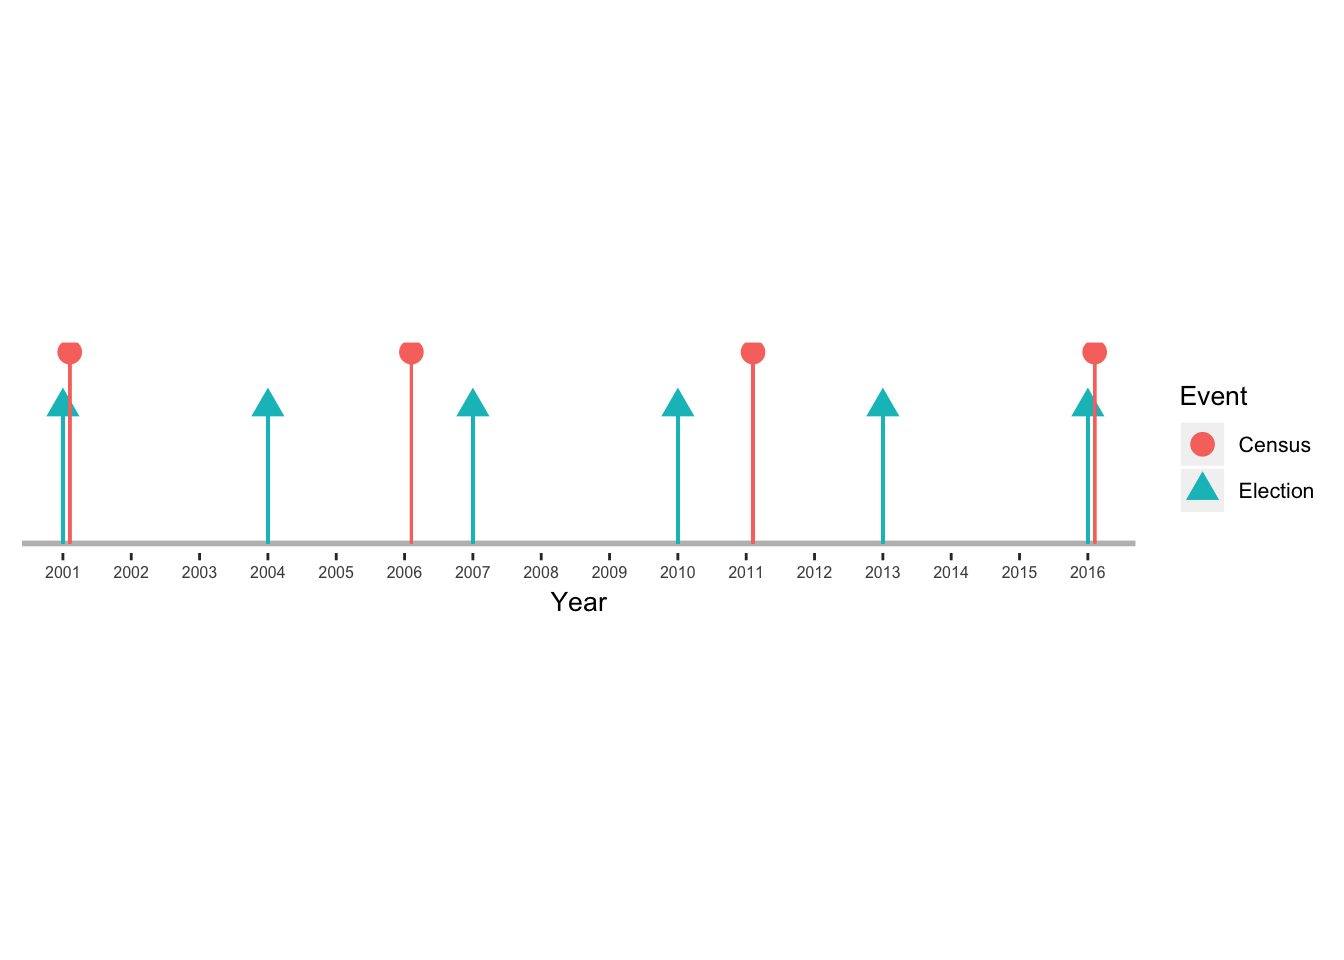
\includegraphics[width=0.9\linewidth]{electoral-modelling-draft_files/figure-latex/timeline-1} 

}

\caption{Timeline of Australian elections and Censuses. They do not always occur in the same year.}\label{fig:timeline}
\end{figure}

\hypertarget{spatio-temporal-imputation}{%
\subsection{Spatio-temporal imputation}\label{spatio-temporal-imputation}}

To account for spatial differences, the piece-wise approximation method in \citet{Goodchild1993} is adopted. Consider a map of source zones \(s = 1,...,S\), for which socio-demographic information is available, and a set of target zones \(t = 1,...,T\) for which information is to be imputed. In this context the map of electoral boundaries at the time of a Census would be the source zones, and the boundaries at the time of the election would be the target zones. Denote the area of intersection between source zone \(s\) and target zone \(t\) as \(A_{s,t}\), the population of the source zone \(s\) as \(U_s\), and the population of intersection between source zone \(s\) and target zone \(t\) as \(P_{s,t}\).

Compute each \(A_{s,t}\) and estimate population of the intersection:

\[\hat{P}_{s,t} = \frac{U_s*A_{s,t}}{\sum_{t=1}^T A_{s,t}}\]
This assumes that populations are uniformly distributed within each source zone.

In order to calculate socio-demographic information for each of the target zones, a weighted average is taken using the estimated population as weights. Denote a given Census variable for the target zone \(C_t\), and the same Census variable for the source zone \(D_s\):

\[\hat{C}_t = \frac{\sum_{s=1}^{S}{D_s*\hat{P}_{s,t}}}{\sum_{s=1}^{S}{\hat{P}_{s,t}}}\]
This assumes that each individual in a source zone assumes the aggregate characteristics of the zone.

Applying this to each of the target zones addresses the spatial component, as it imputes the required socio-demographic for the desired electoral boundaries. However these are applicable at the time of the Census (source year) and are not yet appropriate for the election (target year).

Denote year \(y\), with a Census falling on \(y_1\) and \(y_3\), and an election on year \(y_2\), and add this subscript to the Census variable estimate, \(\hat{C}_{t,y}\). To account for temporal changes, linear interpolation is used between Census years to get the final estimate of a Census variable for the target zone in the election year \(y_2\). This assumes that population evolves in a linear manner over time.

\[\hat{C}_{t,y_2} = \frac{y_3-y_2}{y_3-y_1}*\hat{C}_{t,y_1} + \frac{y_2-y_1}{y_3-y_1}*\hat{C}_{t,y_3}\]

\hypertarget{applied}{%
\subsection{Applied}\label{applied}}

Publically available Census data is aggregated and there are different resolutions accessible, ranging from SA1 (over 50,000 zones) to electoral divisions (150 zones). For this study electoral divisions are used as source zones, and this imputation method is applied for each of the 2004, 2007, 2010 and 2013 elections. To demonstrate its functionality, consider the imputation of socio-demographic variables for the electorate of Hume in New South Wales (NSW), at the time of the 2013 federal election. Figure \ref{fig:hume13} shows this region amongst other NSW electorates.

\begin{figure}[h]

{\centering 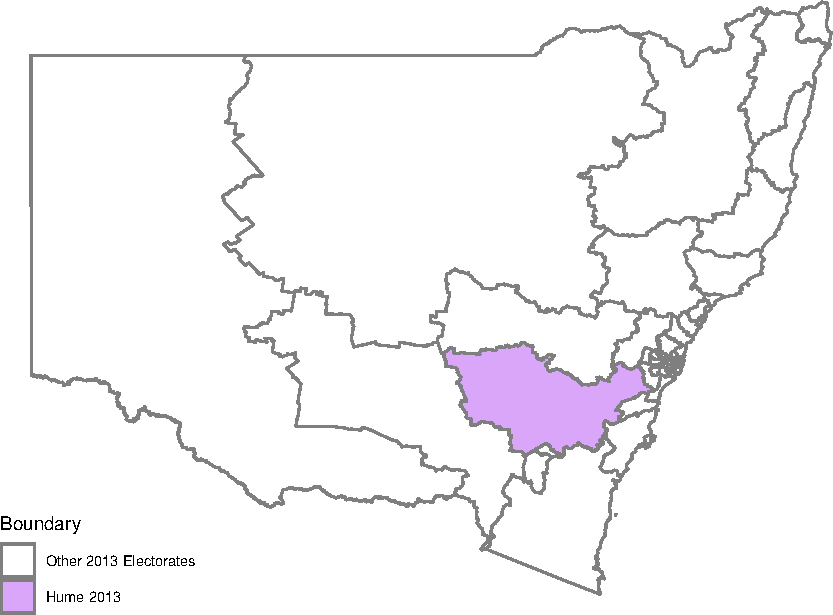
\includegraphics[height=0.3\textheight]{electoral-modelling-draft_files/figure-latex/hume13-1} 

}

\caption{Some of the electoral boundaries in NSW for 2013, with the electoral boundary for Hume, shown in purple.}\label{fig:hume13}
\end{figure}

The Censuses neighbouring the 2013 election are those in 2011 and 2016, and the Hume boundary is changed, as seen by plotting the Hume boundary (purple) in the 2013 election over the divisions in 2016 (see Figure \ref{fig:hume16}).

\begin{figure}[h]

{\centering 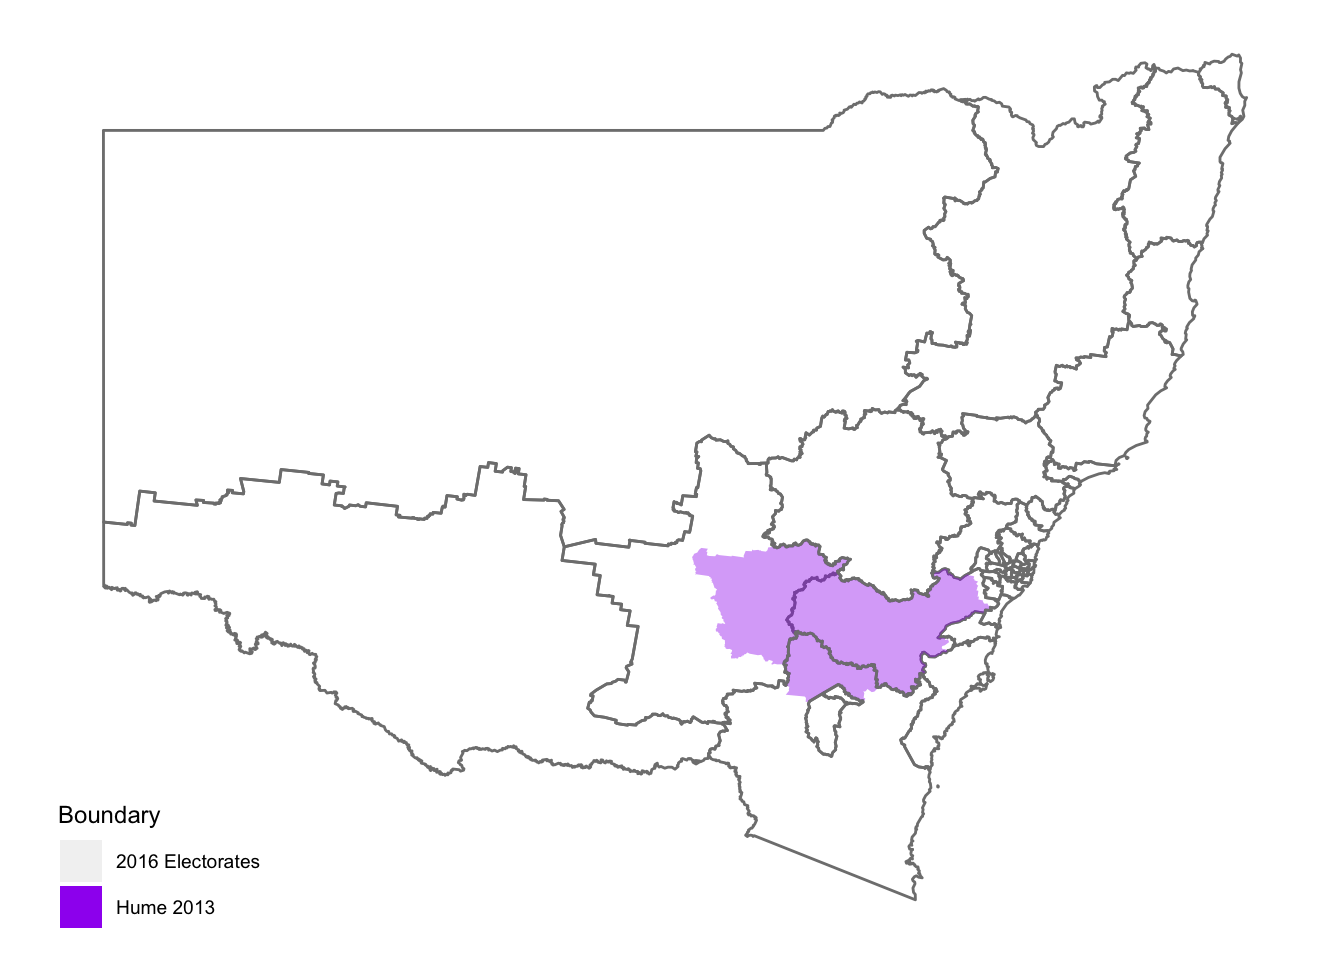
\includegraphics[height=0.3\textheight]{electoral-modelling-draft_files/figure-latex/hume16-1} 

}

\caption{Census division boundaries in NSW for 2016, with the 2013 electoral boundary for Hume, shown in purple. The purple region is not contained within a single Census division.}\label{fig:hume16}
\end{figure}

There are many electorates in 2016 that intersect with the purple region (Hume boundary for 2013), these include the divisions of Riverina, Eden-Monaro and Hume, along with smaller intersecting areas with Fenner, Calare, Gilmore and Whitlam. To impute Census information for this purple region, calculate the percentage of each 2016 electorate that intersects with the purple region, which is then used to estimate intersection populations \(\hat{P}_{s,t}\).

\begin{longtable}[]{@{}llll@{}}
\toprule
\begin{minipage}[b]{0.17\columnwidth}\raggedright
Electorate (2016)\strut
\end{minipage} & \begin{minipage}[b]{0.10\columnwidth}\raggedright
Percentage\strut
\end{minipage} & \begin{minipage}[b]{0.22\columnwidth}\raggedright
Population in Electorate\strut
\end{minipage} & \begin{minipage}[b]{0.40\columnwidth}\raggedright
Estimated Population Allocated to Purple Region: \(\hat{P}_{s,t}\)\strut
\end{minipage}\tabularnewline
\midrule
\endhead
\begin{minipage}[t]{0.17\columnwidth}\raggedright
HUME\strut
\end{minipage} & \begin{minipage}[t]{0.10\columnwidth}\raggedright
96.54\%\strut
\end{minipage} & \begin{minipage}[t]{0.22\columnwidth}\raggedright
150643\strut
\end{minipage} & \begin{minipage}[t]{0.40\columnwidth}\raggedright
145427\strut
\end{minipage}\tabularnewline
\begin{minipage}[t]{0.17\columnwidth}\raggedright
RIVERINA\strut
\end{minipage} & \begin{minipage}[t]{0.10\columnwidth}\raggedright
25.11\%\strut
\end{minipage} & \begin{minipage}[t]{0.22\columnwidth}\raggedright
155793\strut
\end{minipage} & \begin{minipage}[t]{0.40\columnwidth}\raggedright
39117\strut
\end{minipage}\tabularnewline
\begin{minipage}[t]{0.17\columnwidth}\raggedright
EDEN-MONARO\strut
\end{minipage} & \begin{minipage}[t]{0.10\columnwidth}\raggedright
11.09\%\strut
\end{minipage} & \begin{minipage}[t]{0.22\columnwidth}\raggedright
147532\strut
\end{minipage} & \begin{minipage}[t]{0.40\columnwidth}\raggedright
16358\strut
\end{minipage}\tabularnewline
\begin{minipage}[t]{0.17\columnwidth}\raggedright
CANBERRA\strut
\end{minipage} & \begin{minipage}[t]{0.10\columnwidth}\raggedright
0.28\%\strut
\end{minipage} & \begin{minipage}[t]{0.22\columnwidth}\raggedright
196037\strut
\end{minipage} & \begin{minipage}[t]{0.40\columnwidth}\raggedright
548\strut
\end{minipage}\tabularnewline
\begin{minipage}[t]{0.17\columnwidth}\raggedright
FENNER\strut
\end{minipage} & \begin{minipage}[t]{0.10\columnwidth}\raggedright
0.23\%\strut
\end{minipage} & \begin{minipage}[t]{0.22\columnwidth}\raggedright
202955\strut
\end{minipage} & \begin{minipage}[t]{0.40\columnwidth}\raggedright
474\strut
\end{minipage}\tabularnewline
\begin{minipage}[t]{0.17\columnwidth}\raggedright
WHITLAM\strut
\end{minipage} & \begin{minipage}[t]{0.10\columnwidth}\raggedright
0.06\%\strut
\end{minipage} & \begin{minipage}[t]{0.22\columnwidth}\raggedright
152280\strut
\end{minipage} & \begin{minipage}[t]{0.40\columnwidth}\raggedright
92\strut
\end{minipage}\tabularnewline
\begin{minipage}[t]{0.17\columnwidth}\raggedright
GILMORE\strut
\end{minipage} & \begin{minipage}[t]{0.10\columnwidth}\raggedright
0.06\%\strut
\end{minipage} & \begin{minipage}[t]{0.22\columnwidth}\raggedright
150436\strut
\end{minipage} & \begin{minipage}[t]{0.40\columnwidth}\raggedright
86\strut
\end{minipage}\tabularnewline
\begin{minipage}[t]{0.17\columnwidth}\raggedright
CALARE\strut
\end{minipage} & \begin{minipage}[t]{0.10\columnwidth}\raggedright
0.01\%\strut
\end{minipage} & \begin{minipage}[t]{0.22\columnwidth}\raggedright
161298\strut
\end{minipage} & \begin{minipage}[t]{0.40\columnwidth}\raggedright
21\strut
\end{minipage}\tabularnewline
\bottomrule
\end{longtable}

Now consider the socio-demographic \(AusCitizen\) - the proportion of people in the region who are Australian citizens.

\begin{longtable}[]{@{}lll@{}}
\toprule
\begin{minipage}[b]{0.18\columnwidth}\raggedright
DivisionNm\strut
\end{minipage} & \begin{minipage}[b]{0.21\columnwidth}\raggedright
AusCitizen (\%): \(D_s\)\strut
\end{minipage} & \begin{minipage}[b]{0.53\columnwidth}\raggedright
Estimated Population Allocated to Purple Region: \(\hat{P}_{s,t}\)\strut
\end{minipage}\tabularnewline
\midrule
\endhead
\begin{minipage}[t]{0.18\columnwidth}\raggedright
HUME\strut
\end{minipage} & \begin{minipage}[t]{0.21\columnwidth}\raggedright
90.02\strut
\end{minipage} & \begin{minipage}[t]{0.53\columnwidth}\raggedright
145427\strut
\end{minipage}\tabularnewline
\begin{minipage}[t]{0.18\columnwidth}\raggedright
RIVERINA\strut
\end{minipage} & \begin{minipage}[t]{0.21\columnwidth}\raggedright
89.11\strut
\end{minipage} & \begin{minipage}[t]{0.53\columnwidth}\raggedright
39117\strut
\end{minipage}\tabularnewline
\begin{minipage}[t]{0.18\columnwidth}\raggedright
EDEN-MONARO\strut
\end{minipage} & \begin{minipage}[t]{0.21\columnwidth}\raggedright
88.00\strut
\end{minipage} & \begin{minipage}[t]{0.53\columnwidth}\raggedright
16358\strut
\end{minipage}\tabularnewline
\begin{minipage}[t]{0.18\columnwidth}\raggedright
CANBERRA\strut
\end{minipage} & \begin{minipage}[t]{0.21\columnwidth}\raggedright
85.48\strut
\end{minipage} & \begin{minipage}[t]{0.53\columnwidth}\raggedright
548\strut
\end{minipage}\tabularnewline
\begin{minipage}[t]{0.18\columnwidth}\raggedright
FENNER\strut
\end{minipage} & \begin{minipage}[t]{0.21\columnwidth}\raggedright
83.64\strut
\end{minipage} & \begin{minipage}[t]{0.53\columnwidth}\raggedright
474\strut
\end{minipage}\tabularnewline
\begin{minipage}[t]{0.18\columnwidth}\raggedright
WHITLAM\strut
\end{minipage} & \begin{minipage}[t]{0.21\columnwidth}\raggedright
89.52\strut
\end{minipage} & \begin{minipage}[t]{0.53\columnwidth}\raggedright
92\strut
\end{minipage}\tabularnewline
\begin{minipage}[t]{0.18\columnwidth}\raggedright
GILMORE\strut
\end{minipage} & \begin{minipage}[t]{0.21\columnwidth}\raggedright
89.03\strut
\end{minipage} & \begin{minipage}[t]{0.53\columnwidth}\raggedright
86\strut
\end{minipage}\tabularnewline
\begin{minipage}[t]{0.18\columnwidth}\raggedright
CALARE\strut
\end{minipage} & \begin{minipage}[t]{0.21\columnwidth}\raggedright
87.56\strut
\end{minipage} & \begin{minipage}[t]{0.53\columnwidth}\raggedright
21\strut
\end{minipage}\tabularnewline
\bottomrule
\end{longtable}

Then taking a weighted average of \(AusCitizen\) using the estimated population as weights yields \(\hat{C}_{Hume,2016} = 89.65 \%\). Repeating this process using the 2011 Census and electoral boundaries yields \(\hat{C}_{Hume,2011} = 91.00 \%\)

Finally, linearly interpolate between 2011 and 2016 to arrive at the 2013 estimate:
\begin{eqnarray*}
\hat{C}_{Hume,2013} & = &\frac{3}{5} \cdot \hat{C}_{Hume,2011} + \frac{2}{5} \cdot \hat{C}_{Hume,2016} \\ 
& = & \frac{3}{5} \cdot 91.00 \% + \frac{2}{5} \cdot 89.65 \% \\ 
& = & 90.46 \%
\end{eqnarray*}

This is done for each of the socio-demographic variables, and repeated each of the 2013 electorates.

\hypertarget{modelling}{%
\chapter{Modelling}\label{modelling}}

\hypertarget{data-pre-processing}{%
\section{Data pre-processing}\label{data-pre-processing}}

With socio-demographic information now available for each electorate, each election is joined to the data corresponding with its two-party preferred vote. Socio-demographic variables within each election year are standardized to have mean zero and variance one, to adjust for changing variable scales. For example, inflation-adjusted median rental prices increased across almost all electorates, with median rent of 200 dollars per week placing an electorate in the 90th percentile in 2001, but only the 30th percentile in 2016.

\hypertarget{dimension-reduction}{%
\subsection{Dimension reduction}\label{dimension-reduction}}

With only \(N = 150\) observations (electorates) in each election and \(p = 65\) socio-demographic variables in each cross-section, any model using all variables would face serious problems with multi-collinearity and over-fitting, likely leading to erroneous conclusions regarding variable significance. Therefore a form of dimension reduction is adopted before models are fit.

Socio-demographic variables\footnote{A preliminary step involved removing all age bands, because age is represented by median age, and to remove variables relating to particular denominations of Christianity.} that represent similar information are combined into ``factors'' using principal component analysis (PCA). The scree plots of the principal components for each election all level off after four components, and the loadings of these four components are similar across the elections. Principal components are then computed on the combined set of socio-demographics across all six elections. A factor is created by combining several variables all have large loadings in a particular component and when there is an intuitive reason as to why these variables could represent common information. A loading with magnitude greater than 0.15 is considered large. After computing these sums, each factor is again standardized to have mean zero and variance one, within each election.

Consider the \texttt{Incomes} factor as an illustration. Independent of principal components, we may suspect that median personal income, median household income and median family income are providing similar information about the financial wellbeing of an electorate. Their loadings in the first principal component are large (0.19, 0.21 and 0.22 respectively), which provides the evidence needed to combine these variables into a single factor, which is called \texttt{Incomes}.

This process reduces the predictor set to \(p = 30\).

\hypertarget{model-framework}{%
\section{Model framework}\label{model-framework}}

An identical model specification is used across the six elections, with each election modelled separately. This allows for the socio-demographic effects to be estimated separately for each year, allowing for interpretation of temporal changes in these effects. This is preferable over a single longitudinal model because it avoids any concerns of undue bias stemming from an incorrectly imposed time-varying restriction on any variable. Without such restrictions, a pooled cross-sectional model does not yield any distinct advantage over separate cross-sections. The panel approach is avoided because of how frequently electoral boundaries change, meaning that electorates that have the same name across elections are not guaranteed to represent the same geographical region. Therefore any fixed or random effects models would be difficult to estimate without implementing consistent boundaries, which would requiring further imputation.

For each cross-section, let the response variable be the two-party preferred vote in favour of the Liberal party, denoted \(Y\), with \(Y = 70\) representing a 70\% preference for Liberal, 30\% for Labor. Although \(Y\) lies in the interval \((0,100)\), observed values are never very close to 0 or 100 (minimum \(24.05 \%\) and maximum \(74.90 \%\)), so there is no need to impose the constraint of \(Y \in [0,100]\). Furthermore, the response is found to be spatially correlated in each election (Moran's I test, \(p \le 7\cdot10^{-15}\)). This is expected, as electorates are aggregate spatial units, and hence the spatial structure of the data must modelled appropriately.

The spatial error model \citep{Anselin88} is chosen because captures spatial heterogeneity by incorporating a spatially structured random effect vector \citep{LeSage2009}. In this context, the random effect can be thought of as capturing the unobserved political climate in each electorate, where the climate is correlated with the climate in neighbouring electorates. This functions under the assumption that the climate is independent of electoral socio-demographics, and that an electorate is equally correlated with any electorate that shares a part of its boundary. Spatial weights are calculated in accordance with these assumptions. The spatial error model is specified as follows:

Let \(\rho\) be spatial autoregressive coefficient, \(\boldsymbol v\) be a spherical error term, \({\boldsymbol W}\) be a matrix of spatial weights (containing information about the neighbouring regions), \(\boldsymbol X\) be a matrix of socio-demographic covariates, \(\boldsymbol \beta\) be a vector of regression coefficients and \(\boldsymbol a\) be a spatially structured random effect vector.

\[{\boldsymbol y} = {\boldsymbol X} {\boldsymbol \beta} + {\boldsymbol a}\]
and

\[{\boldsymbol a} = \rho {\boldsymbol W} {\boldsymbol a} + {\boldsymbol v}\]
where

\[{\boldsymbol v} \sim N({\boldsymbol 0}, \sigma^2 {\boldsymbol I_n})\].

so it can be written

\[{\boldsymbol y} = {\boldsymbol X} {\boldsymbol \beta} + ({\boldsymbol I}_n-\rho {\boldsymbol W})^{-1}{\boldsymbol v}\]

Estimation is done using feasible generalized least squares.

Table 3.1 details the resultant estimated model coefficients and their estimated standard errors for each of the six elections. These are interpreted in the next section.

\begin{table}[!htbp] \centering 
  \caption{Estimated model for each of the six elections.} 
  \label{} 
\scriptsize 
\begin{tabular}{@{\extracolsep{1pt}}lcccccc} 
\\[-1.8ex]\hline 
\hline \\[-1.8ex] 
 & \multicolumn{6}{c}{\textit{Dependent variable:}} \\ 
\cline{2-7} 
\\[-1.8ex] & \multicolumn{6}{c}{Two-party preferred vote in favor of the Liberal party} \\ 
 & 2001 & 2004 & 2007 & 2010 & 2013 & 2016 \\ 
\\[-1.8ex] & (1) & (2) & (3) & (4) & (5) & (6)\\ 
\hline \\[-1.8ex] 
 $\rho$ & 0.46$^{***}$ & 0.29$^{*}$ & 0.24 & 0.19 & 0.27$^{*}$ & 0.50$^{***}$ \\ 
  & (0.15) & (0.17) & (0.17) & (0.16) & (0.16) & (0.17) \\ 
  & & & & & & \\ 
 AusCitizen & $-$3.13 & $-$2.64 & $-$2.53 & $-$0.08 & $-$3.40 & $-$1.80 \\ 
  & (2.26) & (2.43) & (2.34) & (2.79) & (2.76) & (2.71) \\ 
  & & & & & & \\ 
 Born\_Asia & 2.22 & $-$0.95 & $-$1.60 & $-$6.83$^{**}$ & $-$3.03 & $-$0.55 \\ 
  & (2.18) & (2.44) & (2.19) & (2.73) & (2.71) & (2.17) \\ 
  & & & & & & \\ 
 Born\_MidEast & $-$1.15 & $-$1.59 & $-$2.01$^{*}$ & $-$2.03 & $-$0.92 & $-$1.44 \\ 
  & (1.07) & (1.20) & (1.11) & (1.27) & (1.24) & (1.13) \\ 
  & & & & & & \\ 
 Born\_SE\_Europe & $-$3.21$^{**}$ & $-$4.24$^{***}$ & $-$3.61$^{***}$ & $-$4.14$^{***}$ & $-$3.69$^{***}$ & $-$2.72$^{***}$ \\ 
  & (1.42) & (1.46) & (1.02) & (1.19) & (1.07) & (0.97) \\ 
  & & & & & & \\ 
 Born\_UK & 0.25 & $-$0.07 & 0.34 & 0.56 & $-$0.09 & $-$1.32 \\ 
  & (1.00) & (0.98) & (0.90) & (1.07) & (1.04) & (1.04) \\ 
  & & & & & & \\ 
 BornElsewhere & $-$5.04 & $-$4.91 & $-$4.13 & 2.35 & $-$5.23 & $-$4.14 \\ 
  & (3.30) & (3.68) & (3.38) & (4.23) & (4.15) & (3.97) \\ 
  & & & & & & \\ 
 Buddhism & $-$0.49 & $-$0.17 & $-$1.37 & $-$0.83 & $-$0.12 & $-$1.60 \\ 
  & (1.39) & (1.61) & (1.61) & (1.80) & (1.68) & (1.56) \\ 
  & & & & & & \\ 
 Christianity & $-$2.48 & $-$1.23 & 0.38 & 0.50 & 2.41 & 1.68 \\ 
  & (1.73) & (1.85) & (1.83) & (1.99) & (1.85) & (1.78) \\ 
  & & & & & & \\ 
 CurrentlyStudying & $-$2.19$^{**}$ & $-$0.13 & 2.06$^{*}$ & 2.12$^{*}$ & 1.15 & $-$0.16 \\ 
  & (0.99) & (1.13) & (1.17) & (1.25) & (1.26) & (1.18) \\ 
  & & & & & & \\ 
 DeFacto & $-$6.44$^{***}$ & $-$5.37$^{**}$ & $-$6.43$^{***}$ & $-$8.07$^{***}$ & $-$6.56$^{**}$ & $-$8.53$^{***}$ \\ 
  & (1.87) & (2.48) & (2.31) & (3.06) & (3.11) & (2.83) \\ 
  & & & & & & \\ 
 DiffAddress & 3.88$^{***}$ & 5.06$^{***}$ & 4.22$^{***}$ & 5.57$^{***}$ & 3.53$^{*}$ & 5.67$^{***}$ \\ 
  & (0.94) & (1.12) & (0.99) & (1.76) & (1.91) & (1.60) \\ 
  & & & & & & \\ 
 Distributive & 1.27 & 2.01$^{*}$ & 1.36 & 1.57 & 2.10$^{*}$ & 1.20 \\ 
  & (1.12) & (1.21) & (1.13) & (1.34) & (1.27) & (1.21) \\ 
  & & & & & & \\ 
 Education & 1.08 & 0.52 & $-$5.52$^{*}$ & $-$4.08 & $-$4.44 & $-$7.07$^{**}$ \\ 
  & (2.38) & (3.12) & (3.27) & (3.95) & (3.78) & (3.55) \\ 
  & & & & & & \\ 
 Extractive & 4.83$^{***}$ & 5.45$^{***}$ & 5.37$^{***}$ & 7.31$^{***}$ & 6.71$^{***}$ & 7.43$^{***}$ \\ 
  & (1.48) & (1.42) & (1.36) & (1.56) & (1.47) & (1.39) \\ 
  & & & & & & \\ 
 FamHouseSize & $-$0.16 & 0.87 & $-$2.40 & $-$2.53 & $-$3.26 & $-$2.91 \\ 
  & (2.19) & (2.72) & (2.69) & (3.25) & (3.28) & (2.90) \\ 
  & & & & & & \\ 
 Incomes & 4.36$^{**}$ & 5.03$^{*}$ & 9.45$^{***}$ & 7.09$^{**}$ & 7.97$^{***}$ & 12.20$^{***}$ \\ 
  & (1.77) & (2.66) & (2.75) & (3.25) & (2.92) & (2.75) \\ 
  & & & & & & \\ 
 Indigenous & 2.91$^{*}$ & 1.97 & 2.48 & 2.84 & 0.67 & $-$0.05 \\ 
  & (1.68) & (1.95) & (1.75) & (2.16) & (2.14) & (2.00) \\ 
  & & & & & & \\ 
 Islam & $-$0.92 & $-$0.97 & $-$0.54 & $-$2.50 & $-$0.82 & $-$0.95 \\ 
  & (1.22) & (1.36) & (1.27) & (1.52) & (1.42) & (1.34) \\ 
  & & & & & & \\ 
 Judaism & 1.88$^{*}$ & 1.78 & 2.66$^{***}$ & 1.97$^{*}$ & 2.74$^{**}$ & 1.65$^{*}$ \\ 
  & (1.05) & (1.13) & (1.01) & (1.15) & (1.10) & (1.00) \\ 
  & & & & & & \\ 
 ManagerAdminClericalSales & 2.06$^{***}$ & 3.32$^{***}$ & 6.00$^{***}$ & 5.47$^{***}$ & 5.04$^{***}$ & 5.78$^{***}$ \\ 
  & (0.71) & (0.93) & (0.90) & (1.08) & (1.03) & (1.06) \\ 
  & & & & & & \\ 
 Married & 0.44 & 0.11 & $-$1.22 & $-$0.22 & 0.91 & $-$2.34 \\ 
  & (2.31) & (2.96) & (2.83) & (3.15) & (3.03) & (2.81) \\ 
  & & & & & & \\ 
 MedianAge & 2.32$^{*}$ & 4.96$^{***}$ & 3.66$^{**}$ & 4.00$^{*}$ & 2.30 & 2.87 \\ 
  & (1.32) & (1.65) & (1.81) & (2.26) & (2.08) & (1.79) \\ 
  & & & & & & \\ 
 NoReligion & $-$1.57 & $-$0.92 & 0.56 & $-$0.30 & 1.02 & 1.31 \\ 
  & (1.59) & (1.71) & (1.73) & (1.92) & (1.94) & (2.04) \\ 
  & & & & & & \\ 
 OneParent\_House & $-$1.73 & $-$0.45 & $-$0.75 & $-$1.46 & $-$0.77 & $-$0.74 \\ 
  & (1.36) & (1.59) & (1.49) & (1.69) & (1.57) & (1.47) \\ 
  & & & & & & \\ 
 OtherLanguageHome & $-$0.44 & 5.92 & 9.98$^{**}$ & 11.24$^{**}$ & 9.00$^{*}$ & 9.84$^{**}$ \\ 
  & (3.22) & (4.16) & (3.91) & (4.76) & (4.66) & (4.44) \\ 
  & & & & & & \\ 
 PropertyOwned & $-$0.46 & $-$0.53 & 0.67 & $-$0.94 & $-$0.48 & 1.41 \\ 
  & (1.37) & (1.50) & (1.43) & (1.76) & (1.67) & (1.50) \\ 
  & & & & & & \\ 
 RentLoanPrice & $-$1.57 & $-$3.32$^{*}$ & $-$4.01$^{**}$ & $-$0.97 & $-$0.70 & $-$0.89 \\ 
  & (1.49) & (1.76) & (1.67) & (2.07) & (2.07) & (2.16) \\ 
  & & & & & & \\ 
 SocialServ & 2.51$^{*}$ & 1.65 & 2.47$^{*}$ & 2.53$^{*}$ & 2.35$^{*}$ & 4.45$^{***}$ \\ 
  & (1.33) & (1.41) & (1.29) & (1.47) & (1.32) & (1.19) \\ 
  & & & & & & \\ 
 Transformative & 3.24$^{**}$ & 4.73$^{***}$ & 4.84$^{***}$ & 4.46$^{**}$ & 3.56$^{**}$ & 4.58$^{***}$ \\ 
  & (1.55) & (1.78) & (1.74) & (1.98) & (1.78) & (1.53) \\ 
  & & & & & & \\ 
 Unemployment & $-$2.45$^{*}$ & $-$3.07$^{*}$ & 0.29 & 0.08 & 1.67 & 2.79$^{**}$ \\ 
  & (1.40) & (1.63) & (1.51) & (1.76) & (1.51) & (1.37) \\ 
  & & & & & & \\ 
 Constant & 50.81$^{***}$ & 52.60$^{***}$ & 47.31$^{***}$ & 49.93$^{***}$ & 53.51$^{***}$ & 50.49$^{***}$ \\ 
  & (0.71) & (0.58) & (0.52) & (0.57) & (0.58) & (0.80) \\ 
  & & & & & & \\ 
\hline \\[-1.8ex] 
Observations & 150 & 150 & 150 & 150 & 150 & 150 \\ 
Residual Standard Error (GLS) & 4.69 & 5.04 & 4.79 & 5.63 & 5.18 & 4.88 \\ 
Log Likelihood & $-$402.11 & $-$410.52 & $-$404.94 & $-$423.96 & $-$412.62 & $-$404.34 \\ 
Akaike Inf. Crit. & 868.21 & 885.05 & 873.88 & 911.92 & 889.24 & 872.68 \\ 
Bayesian Inf. Crit. & 957.14 & 973.98 & 962.81 & 1,000.85 & 978.17 & 961.62 \\ 
\hline 
\hline \\[-1.8ex] 
\textit{Note:}  & \multicolumn{6}{l}{$^{*}$p$<$0.1; $^{**}$p$<$0.05; $^{***}$p$<$0.01} \\ 
 & \multicolumn{6}{l}{Estimated coefficients for variable named in column one shown for} \\ 
 & \multicolumn{6}{l}{election year indicated by column heading, with estimated standard} \\ 
 & \multicolumn{6}{l}{deviation for each coefficient shown below in parenthesis. Overall} \\ 
 & \multicolumn{6}{l}{summary measures for each regression equation are provided in the} \\ 
 & \multicolumn{6}{l}{bottom panel.} \\ 
\end{tabular} 
\end{table}

\hypertarget{results}{%
\chapter{Results}\label{results}}

\hypertarget{spatial-autoregressive-parameter}{%
\section{Spatial autoregressive parameter}\label{spatial-autoregressive-parameter}}

The spatial autoregressive coefficient \(\rho\) is positive and significant in only the 2001 and 2016 elections (Figure \ref{fig:rhovis}), meaning that in these elections, an electorate's political climate was affected by the attitudes of it's neighbours. Conversely, in the other four elections, the spatial effect weakens to become insignficant. In these years, it appears that the spatial component does not explain anything over and above the electoral socio-demographics, meaning electorates voted effectively independently.

\begin{figure}[h]

{\centering 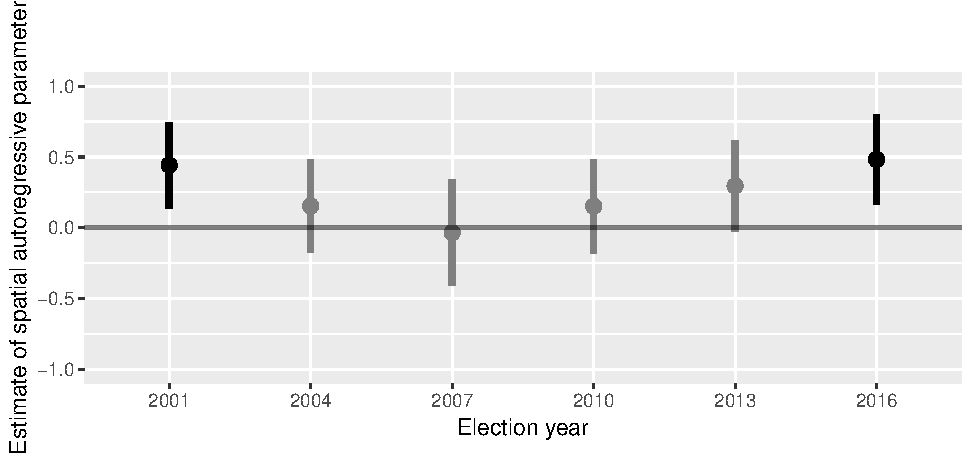
\includegraphics[height=0.2\textheight,]{electoral-modelling-draft_files/figure-latex/rhovis-1} 

}

\caption{Estimates of the spatial autoregressive parameter for each of the six elections, with a 95\% confidence interval. Only in 2001 and 2016 is there a significant spatial component}\label{fig:rhovis}
\end{figure}

\hypertarget{country-wide-trend}{%
\section{Country-wide trend}\label{country-wide-trend}}

Since all socio-demographics have been standardized to have a mean of zero and a variance of one, the intercept in each model can be interpreted as the estimated two-party preferred vote for an electorate with mean characteristics\footnote{Mean of all variables aside from Judaism, Indigenous, Islam and Buddhism, where it assumes the mean of the log value.}. The baseline of party preference has varied over the elections, with the biggest swing occuring in the 2007 election where the mean electorate shifted more than five percentage points in favour of the Labor party.

\begin{figure}[h]

{\centering 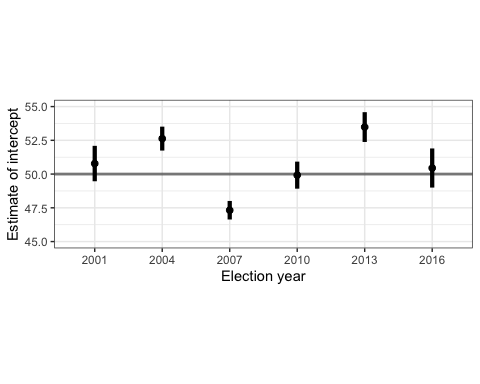
\includegraphics[height=0.2\textheight,]{electoral-modelling-draft_files/figure-latex/plotintercept-1} 

}

\caption{Estimated intercept for each election, which represents the two-party preferred vote for an electorate with mean characteristics.}\label{fig:plotintercept}
\end{figure}

\hypertarget{influential-socio-demographics}{%
\section{Influential socio-demographics}\label{influential-socio-demographics}}

To investigate the socio-demographics that have a strong effect on the two-party preferred vote, partial residual plots are used. These show the direction, size and significance of an estimated effect - the slope of the prediction line matches the estimated coefficient, and the shaded region represents a 95\% confidence band. If a horizontal line can be drawn through the confidence band, then the effect is insignificant. Plots for each election are faceted to compare the effects over time in Figure \ref{fig:partresplot1} and Figure \ref{fig:partresplot2}.

It is important here to note the ecological fallacy - insights are being drawn at the electorate level, and cannot be inferred for another disaggregate level (e.g.~individual voters).

\hypertarget{income-and-unemployment}{%
\subsection{Income and unemployment}\label{income-and-unemployment}}

Typically the Labor party campaigns on more progressive policies, which often include tax reform that adversely affects higher income earners, and more generous social assistance programs. Perhaps due to these policies, higher income electorates have been more likely to support the Liberal party, as the \texttt{Incomes} factor has a positive effect on Liberal preference (see row 1 in Figure \ref{fig:partresplot1}). This effect is signficant in every election aside from 2004, in which it is only marginally insignificant (\(p = 0.0613\)). Unemployment however, has not been as influential. In 2001 and 2004, electorates with higher unemployment were more likely to support Labor, but over time this has shifted towards support for the Liberal party, culminating in a significantly positive effect in 2016.

\hypertarget{industry-and-type-of-work}{%
\subsection{Industry and type of work}\label{industry-and-type-of-work}}

Electorates with higher proportions of workers in mining, gas, water, agriculture, waste and electricity (grouped as \texttt{Extractive} industries) are consistently linked with higher support for the Liberal party, with the mangitude of this effect slightly increasing over the years (see row 3 in Figure \ref{fig:partresplot1}). This is unsurprising, as the Liberal party has close ties with these traditional energy industries, and typically present policies to reduce taxation on energy production. Furthermore, electorates with more workers in construction or manufacturing industries (\texttt{Transformative}) are also more likely to support the Liberal party (see row 4 in Figure \ref{fig:partresplot1}).

Similarly, workers in managerial, administrative, clerical and sales roles (\texttt{ManagerAdminClericalSales}) is also a significant predictor of two-party preference vote across all six elections, with a higher proportion of people working these jobs increasing Liberal support. The magnitude of this effect has also increased over the years.

\hypertarget{household-mobility}{%
\subsection{Household mobility}\label{household-mobility}}

In each of the six elections, electorates with a higher proportion of people that have recently moved house (meaning in last five years) were more likely to support the Liberal party, although this effect was marginally insignificant in 2013 (see row 6 in Figure \ref{fig:partresplot1}. Having controlled for characteristics of house ownership and rental prices (via the factors \texttt{PropertyOwned} and \texttt{RentLoan} respectively), this is effect is somewhat surprising.

\hypertarget{relationships}{%
\subsection{Relationships}\label{relationships}}

De facto relationships, but not marriages, are found to be an important (and significant) predictor of the two-party preferred vote in all six elections, with more de facto relationships associated with higher support for the Labor party. Marriages however, are insignficiant.

\hypertarget{age}{%
\subsection{Age}\label{age}}

Older regions are often believed to be more conservative, and it can be seen that electorates with a higher median age have been more likely to support the Liberal party - although this effect is only significant in 2007 and 2010 (see row 2 in Figure \ref{fig:partresplot2}).

\hypertarget{education}{%
\subsection{Education}\label{education}}

Since 2007, electorates with higher education levels have been associated with supporting the Labor party, although this effect is only significant in 2016. Prior to 2007, education had an almost zero effect (see row 3 in \ref{fig:partresplot1}).

\hypertarget{diversity}{%
\subsection{Diversity}\label{diversity}}

Larger migrant populations from Asia, the Middle East, South-Eastern Europe, the United Kingdom and elsewhere, are either assocated with Labor support, or have no effect. Of these areas, only South-Eastern European populations were signficant in each election and Asian migrants were a significant in 2010. Speaking other language (aside from English) however, have a far stronger effect, as observed through \texttt{OtherLanguageHome}. Electorates with more diverse speech were more likely to support the Liberal party from 2004 onwards, with this effect being significant in 2007, 2010 and 2016. Furthermore, of the variables relating to religion, only Judaism shows a consistent effect, with electorates with larger Jewish populations more likely to vote Liberal.

\hypertarget{partial-residual-plots}{%
\subsection{Partial residual plots}\label{partial-residual-plots}}

\begin{figure}[h]

{\centering 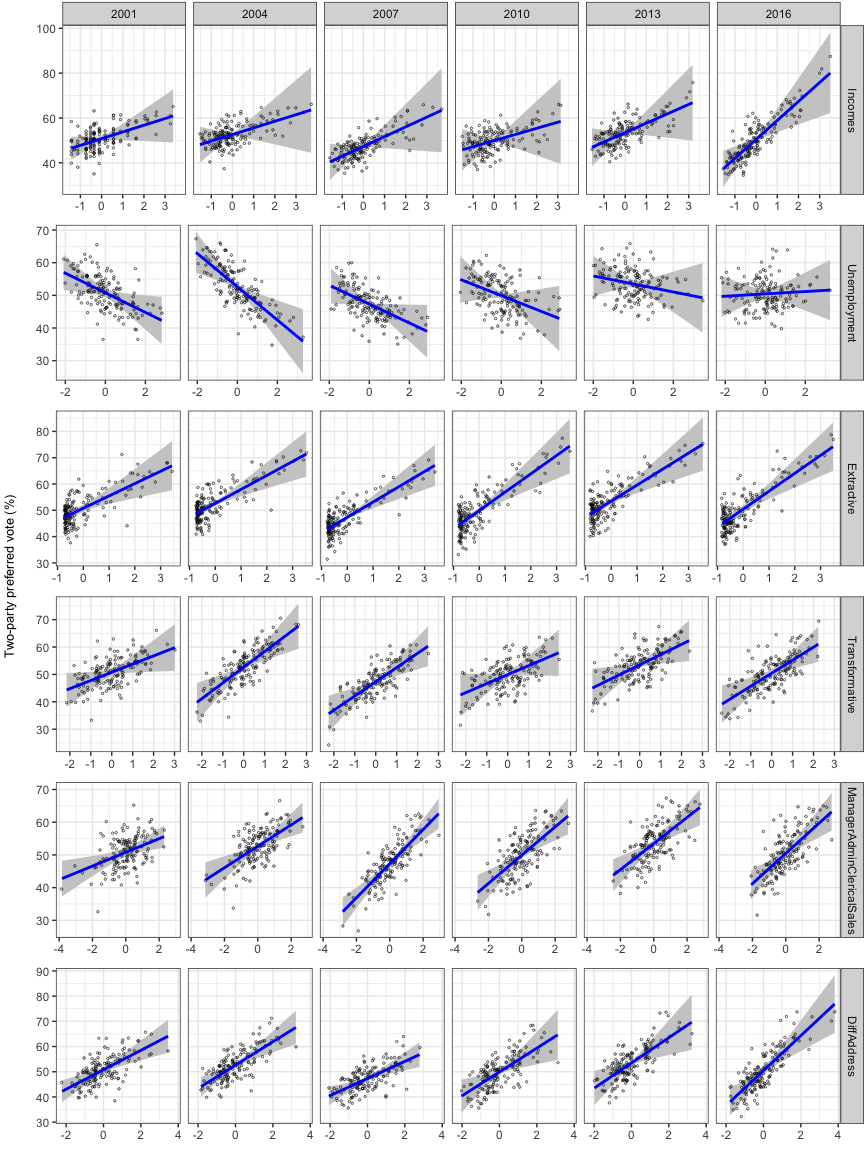
\includegraphics{electoral-modelling-draft_files/figure-latex/partresplot1-1} 

}

\caption{Partial residual plots for: income and unemployment, industry and type of work, and household mobility.}\label{fig:partresplot1}
\end{figure}

\begin{figure}[h]

{\centering 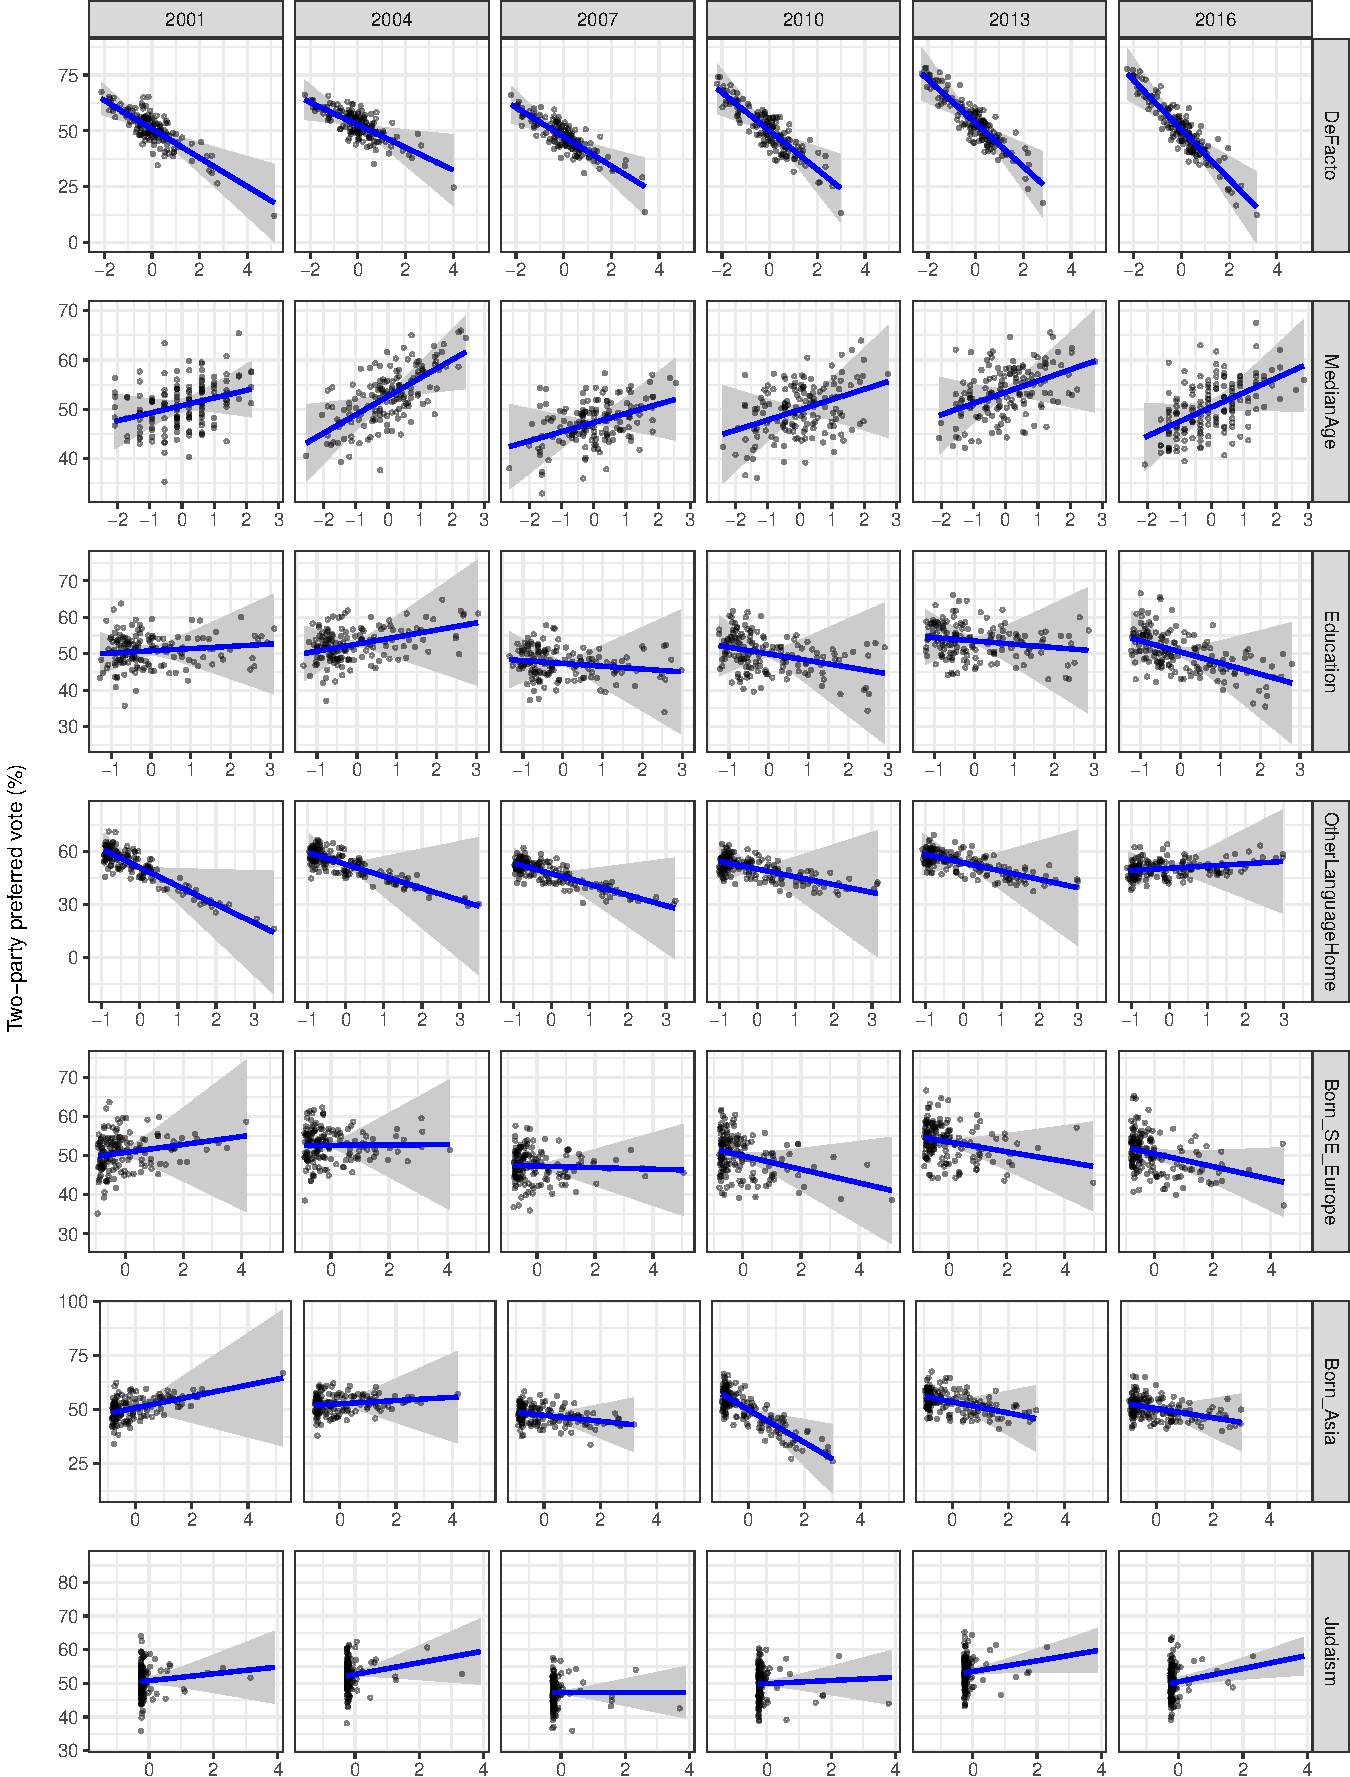
\includegraphics{electoral-modelling-draft_files/figure-latex/partresplot2-1} 

}

\caption{Partial residual plots for: relationships and age, education and diversity.}\label{fig:partresplot2}
\end{figure}

\hypertarget{a-note-on-similar-variables}{%
\subsection{A note on similar variables}\label{a-note-on-similar-variables}}

Many of the Census variables represent similar information, which is why factors were created and some variables were removed. However, there still remain some variables which are closely related. For example, electorate income levels (via \texttt{Incomes}) is likely to be related to electoral unemployment and labor force participation (via \texttt{Unemployment}). In 2001, the coefficient estiamte for \texttt{Unemployment} negative but not significant, and the \texttt{Incomes} variables is significant. If the \texttt{Incomes} variable is removed from the model, \texttt{Unemployment} absorbs the negative effect, becoming significant (\(p = 0.0056\)).

\hypertarget{a-closer-look-at-the-residuals}{%
\section{A closer look at the residuals}\label{a-closer-look-at-the-residuals}}

\hypertarget{residuals-by-state}{%
\subsection{Residuals by state}\label{residuals-by-state}}

It is often hypothesized that states have systematic differences that cause their electorates to vote differently. Boxplots of residuals grouped by state reveal that only Tasmania, the Australian Capital Territory and the Northern Territory appear to have a state-specific effect that is not captured by the models. Tasmania and the Australian Capital Territory appear to have a bias towards Labor, whereas the Northern Territory has one towards Liberal. There are few electorates in these states (five, two and two respectively), so this might be due to incumbent effects rather than an actual state-specific bias.

\begin{figure}[h]

{\centering 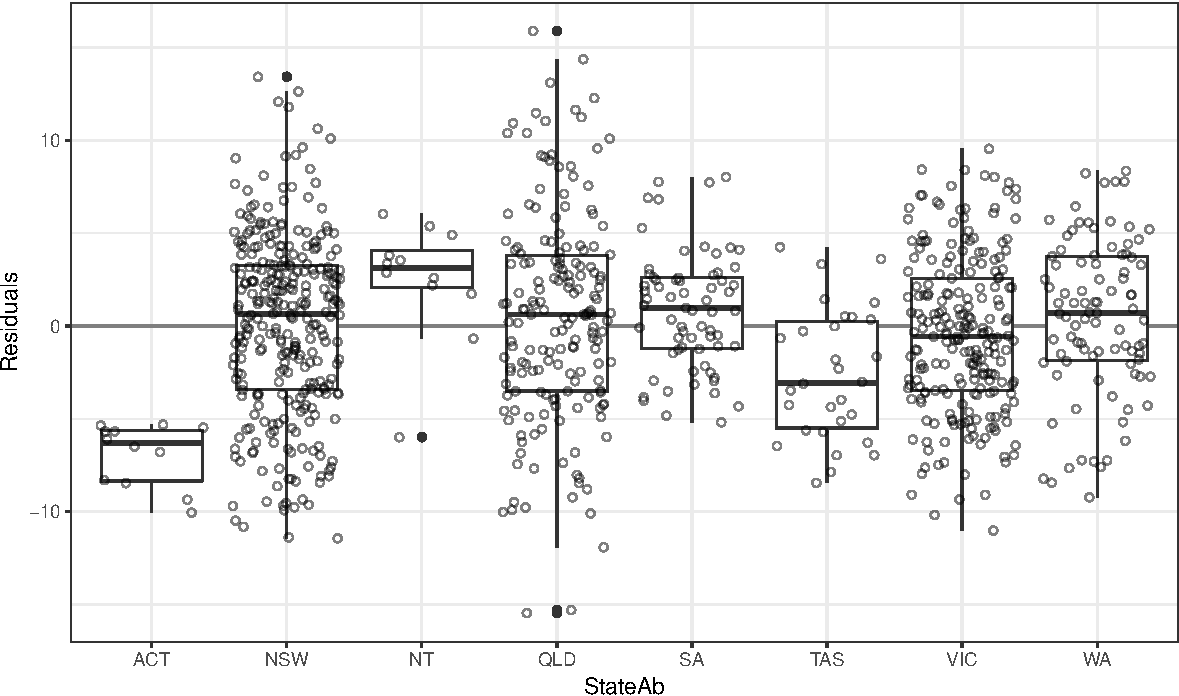
\includegraphics[width=0.8\linewidth,]{electoral-modelling-draft_files/figure-latex/resstate-1} 

}

\caption{Boxplot of residuals by state with jittered points.}\label{fig:resstate}
\end{figure}

\hypertarget{outlier-electorates}{%
\subsection{Outlier electorates}\label{outlier-electorates}}

Based on the distribution of the cook's distance values, a cook's distance greater than \(0.1\) is considered to be influential and a potential outlier. The electorate of Sydney (NSW) has a large cook's distance from 2001 to 2013, due to its diverse population (language, birthplace and religion), high number of defacto relationships, high income, high household mobility and small amount of workers in extractive and transformative jobs. It has remained a strong supporter of the Labor party and Liberal vote is severely overpredicted by the model, making it an outlier. Nearby in metropolitan NSW, the electorate of Wentworth is found to be an outlier in all but the 2007 election. Although historically Liberal, its two-party vote jumped by over 10 percentage points in 2010 without experiencing any notable changes in its socio-demographic makeup - implying that this may be the direct effect of its Liberal member, Malcolm Turnbull, becoming the leader of the Liberal party. Liberal support in Wentworth is underpredicted by the model in each year, and more so with Turnbull as Liberal leader.

Lingiari, an electorate taking up almost all of the Northern Territory, is an outlier in the 2001-2007 elections due to its large Indigenous population, young age profile and low rates of property ownership. Fowler (NSW) has a diverse population with a high proportion of migrants, many Buddhists and Muslims, and has very strong Labor support, making it influential in 2001, 2004 and 2010. Other electorates with large cook's distance are Barton (NSW) and Leichhardt (QLD) in 2016, and Canberra (ACT) in 2007.

\hypertarget{conclusion}{%
\chapter{Conclusion}\label{conclusion}}

Across the past six elections, most of the socio-demographics that drive the electoral two-party preferred vote have remained steady, whilst a few (typically weaker) effects have varied over time. Industry and type of work are particularly influential, with energy-related and manufacturing/construction jobs, as well as administrative roles being strongly linked with the Liberal party in all elections. Incomes have had a similarly consistent effect, with higher income areas supporting Liberal. Higher levels of unemployment have shifted from weak association with Labor to a significant Liberal effect over the years, and higher education levels have been associated with Labor since 2007 (although only significant in 2016). It is also found that electorates with higher household mobility support Liberal, birthplace diversity favours Labor and more de facto relationships align with Labor preference - although marriages, family and household sizes have no material influence. Furthermore, the neighbourhood (spatial) effects were found to be positive in all elections, although only significant in 2001 and 2016, meaning that in the 2004-2013 elections, electorates effectively voted independently.

The findings in this paper complement the existing literature by modelling temporal trends, which as far as the authors are aware, has not been done previously for Australian elections using a regression framework. It is also the first study to model any Australian election since 2010 using Census information. Additionally, a key contribution of this research is the spatio-temporal imputation, which is applied to obtain Census data for the 2004, 2007, 2010 and 2013 elections. All data sets used in this study have been contributed to the \texttt{eechidna} \texttt{R} package, which provides a rich, accessible data resource for future Australian electoral analysis.

\hypertarget{acknowledgements}{%
\chapter{Acknowledgements}\label{acknowledgements}}

This paper was produced using \texttt{RMarkdown}\citep{rmarkdown} and \texttt{knitr} \citep{knitr}. All corresponding code for this paper can be found in the github repository (\url{https://github.com/jforbes14/journal-writing}), and the data used is available in the \texttt{eechidna} package \citep{eechidna}. All raw data was obtained from the Australian Electoral Commission, the Australian Bureau of Statistics and the Australian Government.

\hypertarget{software}{%
\chapter{Software}\label{software}}

All election and Census data sets, along with electoral maps and more, are available in the \texttt{eechidna} \texttt{R} package, which can be downloaded from CRAN. \texttt{eechidna} (Exploring Election and Census Highly Informative Data Nationally for Australia) makes it easy to look at the data from the Australian Federal elections and Censuses that occurred between 2001 and 2016. This study contributed a large revision to the \texttt{eechidna} package, which included the addition of election and Census data for 2001-2010, vote outcomes for polling booths and imputed Census data for election years. For more details on using \texttt{eechidna}, please see the articles (vignettes) on the github page (\url{https://ropenscilabs.github.io/eechidna/}).

The authors would like to give a sincere thanks to Anthony Ebert, Heike Hofmann, Thomas Lumley, Ben Marwick, Carson Sievert, Mingzhu Sun, Dilini Talagala, Nicholas Tierney, Nathaniel Tomasetti, Earo Wang and Fang Zhou, all of whom have contributed to the \texttt{eechidna} package.

\bibliography{book.bib,packages.bib}


\end{document}
